\title{คาบเรียนที่ 5: อนุพันธ์}
\frame{\titlepage}


\begin{frame}
\frametitle{สารบัญ}
\tableofcontents
\end{frame}

%%%%%%%%%%%%%%
\section{นิยามของอนุพันธ์}
\frame{\sectionpage}
%%%%%%%%%%%%%%

\begin{frame}
\frametitle{ที่มา}
\addfig{0.7}{diff_motivation_reflection}{สามารถคาดเดาได้หรือไม่ว่าลูกบอลจะสะท้อนไปทางใด}{}
\end{frame}

\begin{frame}[t]
\frametitle{โจทย์การหาความเปลี่ยนแปลง}
เราสามารถเขียนโจทย์เป็นภาษาคณิตศาสตร์ได้ดังนี้
\begin{slide}
\begin{remark}{}
กำหนดสิ่งต่อไปนี้ให้
\begin{itemize}
\item ฟังก์ชัน $f(x)$ 
\item กราฟของฟังก์ชัน $y=f(x)$
\item จุด $P = (x_0, f(x_0))$ ซึ่งอยู่บนกราฟ
\end{itemize}

จงหาความชันของเส้นสัมผัสเส้นโค้ง ณ จุด $P$
\end{remark}
\end{slide}
\end{frame}

\begin{frame}

\begin{figure}[h!]
\centering
\begin{tikzpicture}[domain = -1:3, scale = 2]
\draw[<->] (-0.5,0) -- (3.2,0) node [right] {$x$};
\draw[<->] (0,-0.5) -- (0,2.2) node [above] {$y$};
\draw[dashed] (0.5,-0.5) -- (3,2);
\filldraw[fill = red] (2,1) circle (1pt) node [left] {$(x,y) = (2,1)$};
\draw[very thick, blue] plot (\x, \x*\x/4) node [right, scale = 2] {$y = \frac{x^2}{4}$};
\end{tikzpicture}
\caption{ภาพแสดงฟังก์ชัน $y=\frac{x^2}{4}$ และเส้นสัมผัส (เส้นประ) ที่จุด $(x,y) = (2,1)$}
\end{figure}
\end{frame}

\begin{frame}
เนื่องจากเรายังไม่ทราบวิธีการสร้างเส้นสัมผัส เราจึงเริ่มจากสร้างเส้นตรงโดยการเลือกจุด $Q$ อีกจุดที่อยู่บนกราฟเช่นกัน และสร้างส่วนของเส้นตรง $PQ$ ขึ้นมา

\begin{figure}[h!]
\centering
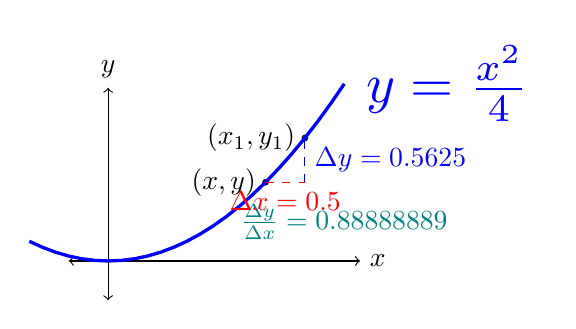
\begin{tikzpicture}[domain = -1:3]
\draw[<->] (-0.5,0) -- (3.2,0) node [right] {$x$};
\draw[<->] (0,-0.5) -- (0,2.2) node [above] {$y$};
\filldraw[fill = red] (2,1) circle (1pt) node [left] {$(x,y)$};
\filldraw[fill = teal] (2.5,1.5625) circle (1pt) node [left] {$(x_1,y_1)$};
\draw[very thick, blue] plot (\x, \x*\x/4) node [right, scale = 2] {$y = \frac{x^2}{4}$};
\draw[red, dashed] (2,1) -- (2.5,1) node [below, pos=0.5] {$\Delta x = 0.5$}; 
\draw[blue, dashed] (2.5,1) -- (2.5,1.5625) node [right, pos=0.5] {$\Delta y = 0.5625$};
\node at (3,0.5) [teal] {$\frac{\Delta y}{\Delta x} = 0.88888889$};
\end{tikzpicture}
\caption{ภาพแสดงการหาความชันของเส้นตรงที่เชื่อมจุด $(x,y)$ และ $(x_1,y_1)$}
\end{figure}
\end{frame}

\begin{frame}
\begin{slide}
จากรูป จะเห็นว่า ความชันของเส้นตรงที่ผ่านจุด $P$ และ $Q$  คือ
\[ \frac{\Delta y}{\Delta x} = \frac{f(x+h) - f(x)}{h}\]   
ถ้าให้  $h$ เข้าใกล้ 0 (ทางซ้ายและทางขวา) จะได้ว่า จุด $Q$  เคลื่อนที่เข้าหาจุด $P$  จนทำให้ส่วนของเส้นตรง $PQ$  เข้าใกล้เส้นสัมผัสเส้นโค้ง $y=f(x)$ ที่จุด $P$ 
\medskip 

ดังนั้นความชันของเส้นสัมผัสเส้นโค้ง  $y=f(x)$ ที่จุด $x$  ใดๆ คือ
\[ \limh \frac{f(x+h) - f(x)}{h}\]
\end{slide}
\end{frame}


\begin{frame}
\frametitle{นิยามของอนุพันธ์}
\begin{defn}{}{}
ให้  $f$ เป็นฟังก์ชันของตัวแปร $x$ โดยที่ $y = f(x)$ แล้ว ฟังก์ชัน $f$ จะเรียกว่า \textbf{หาอนุพันธ์ได้ที่จุด} $\mathbf{x}$  ก็ต่อเมื่อ    
\begin{equation}
\limh \frac{f(x+h) - f(x)}{h}
\end{equation}
หาค่าได้ \pa ถ้าลิมิตหาค่าได้ เราเรียกว่า อนุพันธ์ของ $f$  ที่ $x$  และเขียนแทนด้วยสัญลักษณ์ใดสัญลักษณ์หนึ่งต่อไปนี้
\[ \dx f(x) = \limh \frac{f(x+h) - f(x)}{h}\]
\end{defn}
\end{frame}


\begin{frame}[t]
\begin{ex}
จงหาอนุพันธ์ของฟังก์ชัน $f(x) = 2x+3$
\end{ex}
\begin{sol}
\pa หาลิมิตจากสมการ เมื่อแทนค่า $f(x) = 2x+3$ จะได้
\begin{eqnarray*}
\limh \frac{f(x+h) - f(x)}{h} \pa &=& \limh \frac{(2(x+h) + 3)) - (2x+3)}{h} \pa \\
&=& \limh \frac{2x+2h+3-2x-3}{h} \pa \\
&=& \limh \frac{2h}{h} \pa \\
&=& \limh 2 \pa  =2 \pa
\end{eqnarray*}
ฉะนั้น $\dx f(x) = 2$
\end{sol}
\end{frame}


\begin{frame}[t]
\begin{ex}
จงหาอนุพันธ์ของฟังก์ชัน $f(x) = x^2$
\end{ex}
\begin{sol}
\pa หาลิมิตจากสมการ เมื่อแทนค่า $f(x) = x^2$ จะได้
\begin{eqnarray*}
\limh \frac{f(x+h) - f(x)}{h}\pa  &=& \limh \frac{(x+h)^2 - x^2}{h} \pa \\
&=& \limh \frac{(x^2+2xh+h^2) - x^2}{h} \pa \\
&=& \limh \frac{2xh + h^2}{h} \pa = \limh 2x+h \pa = 2x\pa
\end{eqnarray*} 
ฉะนั้น $\dx f(x) = 2x$
\end{sol}
\end{frame}


\begin{frame}[t]
\begin{ex}
จงหาอนุพันธ์ของฟังก์ชัน $f(x) = \frac{1}{x}$
\end{ex}
\begin{sol}
\pa หาลิมิตจากสมการ เมื่อแทนค่า $f(x) =\frac{1}{x}$ จะได้
\begin{eqnarray*}
\limh \frac{f(x+h) - f(x)}{h}\pa  &=& \limh \frac{\left(\frac{1}{x+h}\right) - \left(\frac{1}{x}\right)}{h} \pa \\
&=& \limh \frac{\frac{x - (x+h)}{(x+h)x}}{h} \pa = \limh \frac{-h}{h(x+h)x} \pa \\
&=& \limh \frac{-1}{(x+h)x} \pa = -\frac{1}{x^2} \pa
\end{eqnarray*} 
ฉะนั้น $\dx f(x) = -\frac{1}{x^2}$
\end{sol}
\end{frame}

\begin{frame}
\frametitle{การเขียนอนุพันธ์ในรูปแบบอื่น ๆ}
นอกจากรูปแบบ $\dx f(x)$ ในนิยามแล้ว เราสามารถเขียนในรูปแบบอื่นได้ดังต่อไปนี้
\begin{enumerate}
\item $\dyx$ - การเขียนในรูปแบบนี้ สอดคล้องกับนิยามของความชัน $\frac{\Delta y}{\Delta x}$
\item $\frac{df}{dx}$ - ความหมายเดียวกันกับ $\dyx$ โดยที่เรากำหนดให้ $y = f(x)$ 
\item $f\,'(x)$ - แม้ว่าการเขียนแบบนี้จะกระชับ แต่จะติดปัญหาเวลาศึกษาสมบัติต่าง ๆ เช่น เราจะ\textbf{\red{ไม่}}เขียนเป็น $(3x-1)' = 3$ 
\end{enumerate}
\end{frame}

\begin{frame}
\frametitle{การหาค่าของอนุพันธ์}
ผลลัพธ์จากการหาอนุพันธ์เป็นฟังก์ชัน ถ้าเราต้องการหาค่าของอนุพันธ์ที่จุด $x=x_0$ จะเขียนแทนด้วยสัญลักษณ์ต่อไปนี้
\begin{remark}{}
กำหนดฟังก์ชัน $f(x)$ ที่หาอนุพันธ์ ณ จุด $x = x_0$ ได้ แล้วค่าของอนุพันธ์ที่จุด $x=x_0$ จะเขียนแทนด้วย
\[ \dx f(x) \Big|_{x=x_0} \]
หรือ
\[ f\,'(x_0) \]
\end{remark}
\end{frame}


\begin{frame}[t]
\begin{ex}
จงหาอนุพันธ์ของฟังก์ชัน $f(x) = \frac{1}{x}$ ที่จุด 
\begin{tasks}(2)
\task $x = 2$
\task $x = -\frac{1}{3}$
\end{tasks}
\end{ex}
\begin{sol}
\begin{tasks}(1)
\task เราทราบว่า $\dx \frac{1}{x} = -\frac{1}{x^2}$ ฉะนั้น  $\dx \frac{1}{x} \Big|_{x = 1} = -\frac{1}{2^2} = -\frac{1}{4}$

โดยสามารถเขียนในอีกรูปแบบหนึ่งคือ $f\,'(2) = -\frac{1}{4}$
\task เราทราบว่า $\dx \frac{1}{x} = -\frac{1}{x^2}$ ฉะนั้น $\dx \frac{1}{x} \Big|_{x = -\frac{1}{3}} = -\frac{1}{\left(-\frac{1}{3}\right)^2} = -9$

โดยสามารถเขียนในอีกรูปแบบหนึ่งคือ $f\,'\left(-\frac{1}{3}\right) = -9$
\end{tasks}
\end{sol}
\end{frame}

\begin{frame}
\frametitle{ความสัมพันธ์ระหว่างอนุพันธ์และความต่อเนื่อง}

\begin{cor}{}{}
ถ้า $f$ เป็นฟังก์ชันที่มีอนุพันธ์ที่จุด $x = x_0$ แล้ว $f$ จะมีความต่อเนื่องที่จุด $x = x_0$
\end{cor}
\end{frame}

%%%%%%%%%%%%%%%%%%%%%%%
\section[สูตร]{อนุพันธ์ฟังก์ชันพีชคณิตโดยใช้สูตร}
\frame{\sectionpage}
%%%%%%%%%%%%%%%%%%%%%%%

\begin{frame}
\begin{thm}{}{}
\begin{enumerate}
\item ให้ $c$ เป็นค่าคงตัว แล้ว $\dx c = 0$
\item ให้ $n$ เป็นจำนวน\textbf{จริง} ที่ไม่เป็นศูนย์ แล้วจะได้ว่า $\dx x^n = nx^{n-1}$
\end{enumerate}
\end{thm}
ในบางครั้งเราต้องใช้ทักษะการเปลี่ยนรูปเลขชี้กำลัง เพื่อให้เป็นรูป $x^n$ โดยมีสมบัติพื้นฐานต่อไปนี้
\begin{prop}{}{}
\begin{enumerate}
\item $\frac{1}{x^a} = x^{-a} $ เมื่อ $a$ เป็นจำนวนจริงที่ไม่เป็นศูนย์
\item $\sqrt[n]{x} = x^{\frac{1}{n}}$ เมื่อ $n$ เป็นจำนวนจริงบวก
\end{enumerate}
\end{prop}
\end{frame}

\begin{frame}[t]
\begin{ex}
จงแปลงพจน์ต่อไปนี้ ให้อยู่ในรูปของ $x^n$ เมื่อ $n$ เป็นจำนวนจริง
\begin{tasks}(4)
\task $\frac{1}{x^2}$
\task $\frac{1}{x^5}$
\task $\frac{1}{x^{3.5}}$
\task $\frac{1}{x^{-4}}$
\end{tasks}
\end{ex}
\begin{sol}
\begin{tasks}(1)
\task $\frac{1}{x^2} = x^{-2}$
\task $\frac{1}{x^5} = x^{-5}$
\task $\frac{1}{x^{3.5}} = x^{-3.5}$
\task $\frac{1}{x^{-4}} = x^{-(-4)} = x^4$
\end{tasks}
\end{sol}
\end{frame}

\begin{frame}[t]
\begin{ex}
จงแปลงพจน์ต่อไปนี้ ให้อยู่ในรูปของ $x^n$ เมื่อ $n$ เป็นจำนวนจริง
\begin{tasks}(4)
\task $\sqrt{x}$
\task $\sqrt[3]{x}$
\task $\sqrt[5]{x}$
\task $\sqrt[4]{x^3}$
\end{tasks}
\end{ex}
\begin{sol}
\begin{tasks}(1)
\task $\sqrt{x} = x^{\frac{1}{2}}$
\task $\sqrt[3]{x} = x^{\frac{1}{3}}$
\task $\sqrt[5]{x} = x^{\frac{1}{5}}$
\task $\sqrt[4]{x^3} = (x^3)^{\frac{1}{4}} = x^{\frac{3}{4}}$
\end{tasks}
\end{sol}
\end{frame}

\begin{frame}[t]
\begin{ex}
จงแปลงพจน์ต่อไปนี้ ให้อยู่ในรูปของ $x^n$ เมื่อ $n$ เป็นจำนวนจริง
\begin{tasks}(4)
\task $\frac{1}{\sqrt{x}}$
\task $\frac{1}{\sqrt[3]{x}}$
\task $\frac{\sqrt{x}}{x^2}$
\task $\frac{\sqrt[3]{x}}{\sqrt[4]{x}}$
\end{tasks}
\end{ex}
\begin{sol}
\begin{tasks}(1)
\task $\frac{1}{\sqrt{x}} = \frac{1}{x^{\frac{1}{2}}} = x^{-\frac{1}{2}}$
\task $\frac{1}{\sqrt[3]{x}} = \frac{1}{x^{\frac{1}{3}}} = x^{-\frac{1}{3}}$
\task $\frac{\sqrt{x}}{x^2} = \frac{x^{\frac{1}{2}}}{x^2} = x^{\frac{1}{2} - 2} = x^{-\frac{3}{2}}$
\task $\frac{\sqrt[3]{x}}{\sqrt[4]{x}} = \frac{x^{\frac{1}{3}}}{x^{\frac{1}{4}}} = x^{\frac{1}{3} - \frac{1}{4}} = x^{\frac{1}{12}}$
\end{tasks}
\end{sol}
\end{frame}

\begin{frame}[t]
\begin{ex}
จงหาอนุพันธ์ต่อไปนี้
\begin{tasks}(3)
\task $\dx 4$
\task $\dx \frac{1}{2}$
\task $\dx (-5)$
\end{tasks}
\end{ex}
\begin{sol}
\begin{tasks}(1)
\task เนื่องจาก $f(x) = 4$ เป็นฟังก์ชันค่าคงตัว ฉะนั้น $\dx 4 = 0$
\task เนื่องจาก $f(x) = \frac{1}{2}$ เป็นฟังก์ชันค่าคงตัว ฉะนั้น $\dx \frac{1}{2} = 0$
\task เนื่องจาก $f(x) = -5$ เป็นฟังก์ชันค่าคงตัว ฉะนั้น $\dx (-5) = 0$
\end{tasks}
\end{sol}
\end{frame}


\begin{frame}[t]
\begin{ex}
จงหาอนุพันธ์ต่อไปนี้
\begin{tasks}(3)
\task $\dx x^2$
\task $\dx x^3$
\task $\dx x^4$
\end{tasks}
\end{ex}
\begin{sol}
\begin{tasks}(1)
\task $\dx x^{\red{2}} = \red{2} x^{\red{2}-1} = 2x^1 = 2x$
\task $\dx x^{\red{3}} = \red{3} x^{\red{3}-1} = 3x^2 $
\task $\dx x^{\red{4}} = \red{4} x^{\red{4}-1} = 4x^3$
\end{tasks}
\end{sol}
\end{frame}

\begin{frame}[t]
\begin{ex}
จงหาอนุพันธ์ต่อไปนี้
\begin{tasks}(3)
\task $\dx x^{1.5}$
\task $\dx x^{\frac{4}{3}}$
\task $\dx x^{-5}$
\end{tasks}
\end{ex}
\begin{sol}
\begin{tasks}(1)
\task $\dx x^{1.5} = 1.5 x^{1.5 - 1} = 1.5 x^{0.5}$
\task $\dx x^{\frac{4}{3}} = \frac{4}{3} x^{\frac{4}{3} - 1} = \frac{4}{3} x^{\frac{1}{3}}$
\task $\dx x^{-5} = -5 x^{-5-1} = -5x^{-6}$
\end{tasks}
\end{sol}
\end{frame}

\begin{frame}[t]
\begin{ex}
จงหาอนุพันธ์ต่อไปนี้
\begin{tasks}(4)
\task $\dx \left(\frac{1}{x}\right)$
\task $\dx \left(\frac{1}{x^3}\right)$
\task $\dx \left(\frac{1}{x^5}\right)$
\task $\dx \left(\frac{1}{x^{2.5}}\right)$
\end{tasks}
\end{ex}
\begin{sol}
\begin{tasks}(1)
\task $\dx \frac{1}{x} = \dx x^{-1} = -1x^{-1-1} = -x^{-2}$
\task $\dx \frac{1}{x^3} = \dx x^{-3} = -3x^{-3-1} = -3x^{-4}$
\task $\dx \frac{1}{x^5} = \dx x^{-5} = -5x^{-5-1} = -5x^{-6}$
\task $\dx \frac{1}{x^{2.5}} = \dx x^{-2.5} = -2.5x^{-2.5-1} = -2.5x^{-3.5}$
\end{tasks}
\end{sol}
\end{frame}

\begin{frame}[t]
\begin{ex}
จงหาอนุพันธ์ต่อไปนี้
\begin{tasks}(4)
\task $\dx \sqrt{x}$
\task $\dx \sqrt[3]{x}$
\task $\dx \sqrt[4]{x}$
\task $\dx \sqrt[5]{x^3}$
\end{tasks}
\end{ex}
\begin{sol}
\begin{tasks}(1)
\task $\dx \sqrt{x} = \dx x^{\frac{1}{2}} = \frac{1}{2} x^{\frac{1}{2} -1 } = \frac{1}{2} x^{-\frac{1}{2}}$
\task $\dx \sqrt[3]{x} = \dx x^{\frac{1}{3}} = \frac{1}{3} x^{\frac{1}{3} -1 } = \frac{1}{3} x^{-\frac{2}{3}}$
\task $\dx \sqrt[4]{x} = \dx x^{\frac{1}{4}} = \frac{1}{4} x^{\frac{1}{4} -1 } = \frac{1}{4} x^{-\frac{3}{4}}$
\task $\dx \sqrt[5]{x^3} = \dx x^{\frac{3}{5}} = \frac{3}{5} x^{\frac{3}{5} -1 } = \frac{3}{5} x^{-\frac{2}{5}}$
\end{tasks}
\end{sol}
\end{frame}


\begin{frame}[t]
\begin{ex}
จงหาอนุพันธ์ต่อไปนี้
\begin{tasks}(3)
\task $\dx \left(\frac{1}{x^2}\right)$
\task $\dx \left(\frac{1}{\sqrt{x}}\right)$
\task $\dx x$
\end{tasks}
\end{ex}
\begin{sol}
\begin{tasks}(1)
\task $\dx \frac{1}{x^2} = \dx x^{-2} = -2x^{-2-1} = -2x^{-3} = -\frac{2}{x^3}$
\task $\dx \frac{1}{\sqrt{x}} = \dx x^{-\frac{1}{2}} = -\frac{1}{2} x^{-\frac{1}{2} - 1} = - \frac{1}{2} x^{-\frac{3}{2}}$
\task $\dx x = \dx x^1 = 1(x^0) = 1$
\end{tasks}
\end{sol}
\end{frame}

\begin{frame}{}
\begin{remark}{}
สังเกตว่า $\dx x = 1$ มีที่มาจากสูตร $\dx x^n = nx^{n-1}$ ฉะนั้นจึงใช้สูตรได้ แต่ถ้าต้องการแยกออกมาเป็นอีกสูตรหนึ่งก็ได้ จะได้เป็นสูตรพื้นฐานดังนี้
\begin{itemize}
\item $\dx c = 0$ เมื่อ $c$ เป็นค่าคงตัว
\item $\dx x = 1$
\item $\dx x^n = nx^{n-1}$
\end{itemize}
\end{remark}
\end{frame}

%%%%%%%%%%%%%%%%%%%%%%%
\section[บวกและลบ]{สมบัติอนุพันธ์ผลบวกและลบฟังก์ชัน}
\frame{\sectionpage}
%%%%%%%%%%%%%%%%%%%%%%%

\begin{frame}
\frametitle{สมบัติพื้นฐานของอนุพันธ์}
\begin{prop}{}{}
กำหนดให้ $f$ และ $g$ เป็นฟังก์ชันที่หาอนุพันธ์ได้ทุกค่า $x$ ใน $D_f$ (โดเมนของ $f$) และ $c$ เป็นค่าคงตัว แล้ว \pa
\begin{equation}
\dx cf(x) = c \left( \dx f(x)\right)
\end{equation}
\end{prop}
\end{frame}


\begin{frame}[t]
\begin{ex}
จงหาอนุพันธ์ต่อไปนี้
\begin{tasks}(3) 
\task $\dx 3x^2$
\task $\dx 4x^3$
\task $\dx -2x^5$
\end{tasks}
\end{ex}
\begin{sol}
\begin{tasks}(1) 
\task $\dx 3x^2 = 3 \dx x^2 = 3 (2x) = 6x$
\task $\dx 4x^3 = 4 \dx x^3 = 4(3x^2) = 12x^2$
\task $\dx -2x^5 = -2 \dx x^5 = -2(5x^4) = -10x^4$
\end{tasks}
\end{sol}
\end{frame}

\begin{frame}[t]
\begin{ex}
จงหาอนุพันธ์ต่อไปนี้
\begin{tasks}(4) 
\task $\dx \frac{2}{x^3}$
\task $\dx \frac{1}{4x^5}$
\task $\dx 3 \sqrt[6]{x}$
\end{tasks}
\end{ex}
\begin{sol}
\begin{tasks}(1) 
\task $\dx \frac{2}{x^3} = 2 \dx x^{-3} = 2 (-3x^{-3-1}) = -6x^{-4}$
\task $\dx \frac{1}{4x^5} = \frac{1}{4} \dx x^{-5} = \frac{1}{4} (-5x^{-5-1}) = -\frac{5}{4} x^{-6}$
\task $\dx 3 \sqrt[6]{x} = 3 \dx x^{\frac{1}{6}} = 3 \left( \frac{1}{6} x^{\frac{1}{6} - 1} \right) = \frac{1}{2} x^{-\frac{5}{6}}$
\end{tasks}
\end{sol}
\end{frame}

\begin{frame}
\frametitle{สมบัติพื้นฐานของอนุพันธ์}
\begin{prop}{}{}
กำหนดให้ $f$ และ $g$ เป็นฟังก์ชันที่หาอนุพันธ์ได้ทุกค่า $x$ ใน $D_f$ (โดเมนของ $f$) แล้ว \pa

\begin{equation}
\dx (f \pm g)(x) = \dx f(x) \pm \dx g(x)
\end{equation}

\end{prop}
\end{frame}


\begin{frame}[t]
\begin{ex}
จงหาอนุพันธ์ต่อไปนี้
\begin{tasks}(2)
\task $\dx (x^2 -2x)$ 
\task $ \dx (x^5+x^4)$
\end{tasks}
\end{ex}
\begin{sol}
\begin{eqnarray*}
\dx (x^2 - 2x) \pa &=& \dx x^2 - \dx 2x \pa \\
&=& 2x - 2 \pa \\
\dx (x^5 + x^4) \pa &=& \dx x^5 + \dx x^4 \pa \\
&=& 5x^4 + 4x^3
\end{eqnarray*}
\end{sol}
\end{frame}

%%%%%%%%%%%%%%%%%%%%%%%
\section[คูณ]{สมบัติอนุพันธ์ของผลคูณฟังก์ชัน}
\frame{\sectionpage}
%%%%%%%%%%%%%%%%%%%%%%%

\begin{frame}
\frametitle{อนุพันธ์ผลคูณ}
ในบางครั้ง ฟังก์ชันอยู่ในรูปของผลคูณที่ไม่สามารถแยกได้ เช่น
\[ f(x) = x^2 \sin x\]
เราจึงต้องมีทฤษฎีบทสำหรับหาค่าของอนุพันธ์ของฟังก์ชันผลคูณ
\begin{thm}{}{}
กำหนดให้ $u$ และ $v$ เป็นฟังก์ชันที่หาอนุพันธ์ได้ใน $D_f$ (โดเมนของ $f$)  \pa

แล้ว $uv$ เป็นฟังก์ชันที่หาอนุพันธ์ได้และ \pa
\begin{eqnarray}
\dx (uv)(x) \pa &=& u(x) \dx v(x) + v(x) \dx u(x) \pa
\end{eqnarray}
\end{thm}
\end{frame}


\begin{frame}[t]
\begin{ex}
จงหาอนุพันธ์ของ $f(x) = x^3(x+2)$
\end{ex}
\begin{sol}
เขียน $f(x) = u(x) v(x)$ โดยที่ 
\[u(x) = x^3, \qquad v(x) = x+2\]
\pa จะได้ 
\[\dx u(x) = 3x^2, \qquad \dx v(x) = 1\] 
\pa ฉะนั้น
\begin{eqnarray*}
\dx f(x) = \dx (u\cdot v)(x) \pa &=& u(x) \dx v(x) + v(x) \dx u(x) \pa \\
&=& (x^3)(1) + (x+2)(3x^2) \pa \\
&=& x^3 + 3x^3 + 6x^2 \pa \\
&=& 4x^3 + 6x^2
\end{eqnarray*}
\end{sol}
\end{frame}


\begin{frame}[t]
\begin{ex}
จงหาอนุพันธ์ของ $f(x) =(2x+5)(5x-2)$
\end{ex} \pa
\begin{sol}
เขียน $f(x) = u(x) v(x)$ โดยที่ 
\[u(x) = 2x+5, \qquad v(x) = 5x-2\] 
\pa จะได้ 
\[\dx u(x) = 2, \qquad \dx v(x) = 5\] 
\pa ฉะนั้น
\begin{eqnarray*}
\dx f(x) = \dx (uv)(x) \pa &=& u(x)\dx v(x) + v(x)\dx u(x) \pa \\
&=& (2x+5)(5) + (5x-2)(2)\pa \\
&=& 10x+25 + 10x-4 \pa \\
&=& 20x+21
\end{eqnarray*}
\end{sol}
\end{frame}


\begin{frame}[t]
\begin{ex}
จงหาอนุพันธ์ของ $f(x) =(x^5+x)\left(\frac{1}{x^3} + 2\frac{1}{x^2}\right)$
\end{ex} \pa
\begin{sol}
เขียน $f(x) = u(x) v(x)$ โดยที่ 
\[u(x) = x^5+x, \qquad v(x) = x^{-3} + 2x^{-2}\] 
\pa จะได้ 
\[\dx u(x) = 5x^4+1, \qquad \dx v(x) = -3x^{-4} - 4x^{-3}\] 
\pa ฉะนั้น
\begin{eqnarray*}
\dx (uv)(x) \pa &=& u(x)\dx v(x) + v(x)\dx u(x) \pa \\
&=& (x^5+x)(-3x^{-4} - 4x^{-3}) +  (x^{-3} + 2x^{-2})(5x^4+1)\pa \\
&=& (-3x-4x^2-3x^{-3}-4x^{-2})+(5x+x^{-3}+10x^2+2x^{-2}) \pa \\
&=& 6x^2+2x-2x^{-2}-2x^{-3}
\end{eqnarray*}
\end{sol}
\end{frame}

\begin{frame}
\frametitle{สูตรอนุพันธ์ผลคูณแบบย่อ}
ถ้าเราเข้าใจหลักการหาอนุพันธ์ของผลคูณฟังก์ชันแล้ว เราสามารถเขียนย่อในรูปแบบดังต่อไปนี้ได้
\begin{remark}{}
\begin{eqnarray*}
\dx (u\cdot v)(x) &=& u(x)v'(x) + v(x)u'(x) \pa \\
&=& (uv' + vu')(x) 
\end{eqnarray*}
\end{remark}
\end{frame}

%%%%%%%%%%%%%%%%%%%%%%%
\section[หาร]{สมบัติอนุพันธ์ของผลหารฟังก์ชัน}
\frame{\sectionpage}
%%%%%%%%%%%%%%%%%%%%%%%

\begin{frame}
\frametitle{อนุพันธ์ผลหาร}
ในทำนองเดียวกัน ฟังก์ชันที่อยู่ในรูปผลหาร เช่น $f(x) = \frac{x^2}{x+1}$
ก็สามารถหาอนุพันธ์ได้เช่นกัน โดยที่ไม่จำเป็นต้องจัดรูปใหม่
\begin{thm}{}{}
กำหนดให้ $u$ และ $v$ เป็นฟังก์ชันที่หาอนุพันธ์ได้ใน $D_f$ (โดเมนของ $f$)  \pa

แล้ว $\frac{u}{v}$ เป็นฟังก์ชันที่หาอนุพันธ์ได้และ \pa
\begin{eqnarray}
\dx \left(\frac{u}{v} \right)(x) \pa &=& \frac{v(x) \dx u(x) - u(x) \dx v(x)}{(v(x))^2}
\end{eqnarray}
\end{thm}
\end{frame}


\begin{frame}[t]
\begin{ex}
จงหาอนุพันธ์ของ $f(x) =\frac{1}{2x+3}$
\end{ex} \pa
\begin{sol}
เขียน $f(x) = \frac{u(x)}{v(x)}$ โดยที่ $u(x) = 1$ และ $v(x) = 2x+3$ \pa จะได้ 
\[\dx u(x) = 0, \qquad \dx v(x) = 2\] 
ฉะนั้น
\begin{eqnarray*}
\dx f(x) = \dx \left( \frac{u}{v}\right)(x) \pa &=& \frac{v(x)\dx u(x) - u(x)\dx v(x)}{(v(x))^2}\pa \\
&=& \frac{(2x+3)(0) - (1)(2)}{(2x+3)^2}\pa \\
&=& \frac{-2}{(2x+3)^2}
\end{eqnarray*}
\end{sol}
\end{frame}


\begin{frame}[t]
\begin{ex}
จงหาอนุพันธ์ของ $f(x) =\frac{3x+2}{4x-5}$
\end{ex}
\begin{sol}
เขียน $f(x) = \frac{u(x)}{v(x)}$ โดยที่ $u(x) = 3x+2$ และ $v(x) = 4x-5$ \pa จะได้ 
\[\dx u(x) = 3, \qquad \dx v(x) = 4\]
\pa ฉะนั้น
\begin{eqnarray*}
\dx f(x) = \dx \left( \frac{u}{v}\right)(x) \pa &=& \frac{v(x)\dx u(x) - u(x)\dx v(x)}{(v(x))^2}\pa \\
&=& \frac{(4x-5)(3) - (3x+2)(4)}{(4x-5)^2}\pa \\
&=& \frac{(12x-15)-(12x+8)}{(4x-5)^2} \pa = \frac{-23}{(4x-5)^2}
\end{eqnarray*}
\end{sol}
\end{frame}


\begin{frame}[t]
\begin{ex}
จงหาอนุพันธ์ของ $f(x) =\frac{x+1}{x^2+1}$
\end{ex}
\begin{sol}
เขียน $f(x) = \frac{u(x)}{v(x)}$ โดยที่ $u(x) = x+1$ และ $v(x) = x^2+1$ \pa จะได้ 
\[\dx u(x) = 1, \qquad \dx v(x) = 2x\]
\pa ฉะนั้น
\begin{eqnarray*}
\dx f(x) = \dx \left( \frac{u}{v}\right)(x) \pa &=& \frac{v(x)\dx u(x) - u(x) \dx v(x)}{(v(x))^2}\pa \\
&=& \frac{(x^2+1)(1) - (x+1)(2x)}{(x^2+1)^2}\pa \\
&=& \frac{(x^2+1) - (2x^2+2x)}{(x^2+1)^2} \pa = \frac{-x^2-2x+1}{(x^2+1)^2}
\end{eqnarray*}
\end{sol}
\end{frame}

\begin{frame}
\frametitle{สูตรอนุพันธ์ผลหารแบบย่อ}
ในทำนองเดียวกัน เราสามารถเขียนสูตรอนุพันธ์ผลหารแบบย่อได้ดังนี้
\begin{remark}{}
\begin{eqnarray*}
\dx \left(\frac{u}{v} \right)(x) &=& \frac{v(x)u'(x) - u(x)v'(x)}{(v(x))^2}\pa \\
&=& \left( \frac{vu'-uv'}{v^2}\right) (x)
\end{eqnarray*}
\end{remark}
\end{frame}
